%!TEX root=main.tex

% ========
\section{SM-EFT: The Bottom-Up Approach}
\label{sec:classification}

Currently, in particle physics, there are no experimental
results that would allow one to clearly identify any of the 2499 additional possible
dimension-six operators
(see Sec.~\ref{sec:eftintro}) as a signal of BSM physics. 
Instead, only more or less strong upper limits exist.
As we will discuss, the way the SM-EFT is used by physicists can be divided into three different stages.
These stages are used to support the search for BSM both experimentally and theoretically,
with several goals coming together: they serve as accounting scheme both in general and in an approach focussed on a special sector of the SM. 
Thus, they impose constraints on model building and, in case of an indication for a non-vanishing
Wilson coefficient, allow physicists to evaluate potential general consequences and possible 
realizations in a concrete BSM model.

We refer to the SM-EFT with all 2499 dim-6 operators as \emph{Stage 1}.
This stage 1 SM-EFT does not represent a specific new interaction
and thus it has no target in a sense that would allow it to
guide experimental searches.  
If all coefficients $c_i$ in Eq.~\ref{eq:smeft}
were considered to be potentially non-zero, it would allow a virtually infinite number 
of observable distributions (be it interaction rates, asymmetries, kinematic
distributions or any other type of possible particle physics measurement) 
to deviate from the SM without
any specific theoretical preference of what should be experimentally
expected.
This is not sufficient to constitute an experimental target. 
Thus, the stage 1 SM-EFT just serves as a tool to potentially parametrize, or in general
constrain, possible deviations from the SM. 
% which are consistent with the underlying assumptions of the SM-EFT. 

\emph{Stage 2} of the bottom-up approach is an operational response
to the impossibility to theoretically control 2499 parameters or the corresponding experimental distributions simultaneously. 
Instead, physicists typically just focus on a small subset of the SM-EFT and attempt to include all relevant experimental information from one specific experimental sector, prominently undertaken for top quark physics, bottom quark physics (see Section~\ref{sec:Bphysics}), or Higgs physics. 
Such separations between different sectors of the SM
violate gauge invariance, but a reasonable choice of the basis of the
SM-EFT (see Section~\ref{sec:smeftphysics}) alleviates its effect on  
finding deviations at the LHC in the respective sector.
Since currently the strongest focus is on Higgs physics, as a new
and unique potential portal for new physics, let us clarify the stage 2 concept with
this example~\citep{Espinosa:2016ovf,deFlorian:2016spz}.
The number of operators for such dedicated studies are given by a suitable choice
of the basis, their relevance to Higgs couplings,
experimental constraints on the corresponding Wilson coefficients and
possibly by assuming additional symmetries.
While for such a `Higgs EFT' different approaches exist, they typically neglect
four-fermion operators, operators
describing gauge-boson self-interactions, operators for the $W$-mass and 
for the fermion couplings to $Z$ and $W$.
% For example, assuming no additional source of CP violation and assuming
% only flavour-diagonal couplings reduces the number of coefficients to
% 59~\citep{Buchmuller:1985jz,Grzadkowski:2010es}, 
This reduces the number of independent operators to 59, which still far exceeds the experimental capability to set constraints simultaneously on the parameters from separate experimental sectors. 
However, measurements already put significant constraints on several of these parameters, such that for experimental and theoretical studies, only part are considered relevant for LHC physics.
In addition, the number of operators can be reduced to a mere handful by assuming CP conservation or minimal flavour violation.
This reduction to a few parameters is operationally motivated and makes \emph{Stage 2} experimentally and phenomenologically useful by mapping measurements to a manageable set of parameters. 
But even while the number of operators potentially deviating from the SM is reduced, this sectorised SM-EFT still lacks a specific experimental target. 
It only reduces the number of distributions that appear to be a meaningful probe for deviations.
This conclusion is also supported by the current experimental constraints on the Wilson coefficients in the Higgs boson sector: for a model with a clear experimental target, one would expect that experimental results allow one to constrain the allowed range of parameters or to refute the
model. 
However, as shown in~\citep{ATL-PHYS-PUB-2019-042},
the SM-EFT parameters cannot be constrained if more than two Wilson
coefficients are tested at the same time: there are ``flat
directions'' for all parameters, which means that effectively every
parameter can take any value. Therefore, it carries no
\emph{specific} information based on the data.

An EFT analysis obtains a clear target if specific operators are selected, either to account for experimental indications of a new signal, or by specific additional theoretical motivations reaching beyond the logic of the SM-EFT. 
We refer to it as \emph{Stage 3}.  
In such a situation, only a very small set of Wilson coefficients would be considered to be non-zero, such that only few operators are to be considered relevant.
An example of such a situation is given in Section~\ref{sec:BphysicsConcepts}.
In this case, it would be possible to meaningfully reduce the
ambiguities in representation stemming from the different bases. 
The most efficient SM-EFT basis that describes the data with the
smallest set of operators would then represent a small subset of the
possible new effective vertices.  
This is not dissimilar to the
development of the Fermi theory (see~\ref{ssec:Fermi}). 
In the Fermi
theory, one 4-point interaction vertex with one associated coefficient
$c^2=G_F$ is added to the previously known physics in an effective
theory. 
In case of the bottom quark analyses, described in Section~\ref{sec:BphysicsConcepts}, the apparent violation of lepton-flavour universality in the bottom quark sector motivates the use of specific operators to describe observed experimental features, thus they represent specific interactions. 
This is a qualitative difference in Stage 3 with respect to Stages 1 and 2: the SM-EFT no longer describes potential non-resonant deviations from the SM in a non-unique way (as in Stage~2), but in Stage~3, one selected basis of the SM-EFT uniquely describes features that are distinctively different from the SM.

% =======
\subsection{Differences between these Stages}

Differences between these stages highlight issues that will become
relevant for our discussion of the model character of SM-EFT.
Let us first remark that these stages are meant as analytical categories and do not have to be marched through sequentially in actual scientific practice.
For example, in the early 1980s, without reference to
a systematic development of the SM-EFT,~\cite{Eichten:1983hw} proposed,
a model for fermion substructure (`preons') in analogy to the Fermi theory.

The major difference between Stages 1 and partly Stage 2 versus Stage 3 is the (absence) of an underlying specific physics problem:
the SM-EFT of Stage 1 is motivated only by the general and unspecific idea that the SM should be embedded in a larger theoretical framework and the restrictions of Stage 2 are largely motivated by considerations of scientific practice, Stage 3 is built either to understand a measurement beyond the SM, as will be detailed for a current example in Sect.~\ref{sec:BphysicsConcepts}, or by a concrete idea of how BSM should look like, be it the preon-hypothesis of~\cite{Eichten:1983hw} or the violation of baryon number in the framework of Grand Unified Theories (GUTs), as, for example, in~\cite{Weinberg:1979sa}.   
As already discussed in Sect.~\ref{sec:physrepres},
SM-EFT at Stage 1 works as an accounting scheme to quantify deviations
from SM distributions and possibly correlate different operators.
As such, the SM-EFT is a convenient tool to globally assess the status of the SM.
In contrast, selecting one or a few operators in Stage 3 is a step towards the goal of physicists to arrive at a concrete BSM model involving new entities.
The roles of target, prediction, testability, and representation are therefore significantly different in these stages, which can be gleaned, for example, from the paper of~\cite{Weinberg:1979sa}. %rewrite!! 

%Such selection is based on a general idea, as for example~\cite{Weinberg:1979sa} for lepton
%and baryon number violation, or \cite{Eichten:1983hw} for fermion sub--structures, the
%selection might however also be suggested by indications from measurements. 
%As the quotes by physicists in Sect.~\ref{sec:physrepres} show, measuring the Wilson coefficients
%are tools for BSM models that are of interest to physicists.
%Virtually no physicist considers all SM-EFT operators to simultaneously be indicative for BSM. 
In his paper, Weinberg addresses the specific problem of B--L (non-)conservation (B denoting the baryon number, L the lepton number) with GUTs in mind.
Thus, he explicitly neglects the other operators of the SM-EFT because they are of no relevance for his specific target, but he is careful to select dimension-6 operators that do not conserve baryon number. 
From those he derives general constraints for B--L violation, including relations among observables like partial decay widths of baryons.
Weinberg thus starts from Stage 2; from a well-defined theoretical target, which implies an experimental target, viz. proton decay.
Both of these were considered in concrete models before his paper.

On the other hand, Weinberg also makes clear that limitations exist in his EFT approach. 
He immediately emphasizes that B--L non-conservation should be understood better by specific gauge models of baryon decay \citep[p.~1569]{Weinberg:1979sa}.
A derivation of such a model is hardly possible if it should simultaneously address all 2499 operators of the SM-EFT.
Furthermore, Weinberg's paper is sometimes used as an argument for the ability of SM-EFT to predict: in focussing on two specific dimension-5 operators, Weinberg states that these would produce a neutrino mass of roughly ``10$^{-5}$ and 10$^{-1}$ eV''.
Here, Weinberg argues from what we call Stage 3, which we agree, has a target and representational content.
This, however does not mean that an EFT \textit{per se} allows one to predict: to actually arrive at the values for neutrino masses,
Weinberg assumes certain Wilson coefficients, a cut-off scale of 
10$^{14}$ GeV, suggested by the merging of the electromagnetic, weak and strong couplings, and a coupling of $\cal{O}$(1).
Thus, the EFT \textit{simpliciter} points out at most possibilities. 
To provide a quantitative prediction, it has to be supplemented by an additional assumption that comes closer to a concrete model.
The same is true for the preon assumption of~\cite{Eichten:1983hw}: it motivates searches in certain processes, which were anyhow motivated with parametrisations other than EFT, it provides a framework to set constraints on fermion substructure, but, in the absence of a quantitative estimate of observable effects, it does not allow one to definitely rule out substructure. 

The inability of an EFT at any stage to predict without further model assumptions implies that it cannot be meaningfully tested.
While one can certainly look for any kind of deviation the SM-EFT allows, something that is anyhow in the spirit of expecting BSM somewhere, any non-observation of a deviation would not falsify SM-EFT since it does not allow for a quantitative prediction.  
In consequence, the SM-EFT cannot be tested in a meaningful sense; 
a single operator, supplemented by a physics model, can. 

We thus diagnose a major distinction between Stages 1 and 2 and Stage 3 that will be relevant for determining whether and at what stage the EFT is a model. 
At first glance it may be surprising that the SM-EFT, if interpreted as a collection of operators, does not produce a target or have representational character, whereas each individual operator has.
However, we understand this as a breaking of an (virtually) infinite amount of possibilities into just a single one.
As we know from many examples, such a breaking significantly changes the character of the related objects.
  
% \sout{The final point we want to make is the representational content of SM-EFT vs. a single
% operator. [move to 7.3]
% We assume a representation of an object A in a theory/model B to have at least one 
% or a few (measured or measurable) properties of A to be formally included in B.
% \textbf{Needs a philosophically more correct definition}.
% Representation of something thus requires a target to be represented.
% Since we discussed before that SM-EFT lacks such a target, it also has no representational
% value, different to a single selected operator.
% This may at the first glance seems strange if SM-EFT is just considered as a virtually
% infinite collection of single operators. 
% As such it requires a loss of representation by proceeding from one and an infinite number of operators.
% Beyond the arguments given above, let us note that such a loss of quality is not unusual
% in such an expansion.
% Assume a homogeneous plane. 
% While a direction is given by selecting a certain angle, no direction is given by allowing for
% all angles.}


% These considerations imply that the status of an EFT as
% a model cannot be answered just by looking at a Lagrangian. 
%For example, experimental findings or theoretical assumption on the underlying physics
% may imply a concrete representational property of a selection of operators.
% In the following section, an example of an evolving interpretation of a set of statistically partially significant measurements of deviations from the SM in a Stage~3 SM-EFT is given.

 % ===========
\section{Exemplifying Search Concepts in Bottom Physics}\label{sec:BphysicsConcepts}

In Section~\ref{sec:classification}, we discussed a classification
scheme for the SM-EFT, where the experimental status of the theory can
play an important role in the reduction of very many degrees of
freedom to a very small number. The SM-EFT in \emph{Stage~3} thus can
gain representative character through the identification of new
vertices beyond the SM, which represent new types of interactions
between SM particles. One such experimental situation, which has been
emerging over the last years, are precision tests of rare leptonic
decays of $B$ mesons, where lepton universality is
% violated~\citep{Buttazzo:2017ixm} in
% experiments~\citep{Aaij:2019wad,Abdesselam:2019wac,Aaij:2017vbb,Aaij:2015oid,Abdesselam:2019dgh}
violated in experiments
at a statistical significance of around ${\cal O}(3\,\sigma)$ on
average for sensitive single measurements \citep{Aaij:2015oid,Aaij:2017vbb,Aaij:2019wad,Abdesselam:2019dgh,Abdesselam:2019wac,Buttazzo:2017ixm}.
In this section, it is shown how the different BSM approaches are applied to this heavily discussed set of physics processes.

In the SM, the electroweak gauge bosons, $Z$ and $W^\pm$, couple to
the three lepton flavours ($e$, $\mu$, $\tau$) universally (i.e.\ with
the same strength).  Recent measurements of B-meson decays such as
$b \to sl^+l^-$ and $b \to c l \nu$ show hints for the violation of
lepton flavour universality (LFV) (for an overview, see
also~\citep{Albrecht:2018frt}).  As of yet the statistical and systematic
uncertainties are too high to allow firm claims, but if confirmed,
these measurements would provide evidence for BSM physics. To evaluate
LFV, the three approaches introduced in
Section~\ref{sec:eftintro} to evaluate LFV are pursued: concrete
models; Stage~2 and Stage~3 EFTs; and
simplified models. 

% ========
\subsection{Concrete BSM Models}
\label{sec:B-con-BSM}

To explain the apparent LFV with a concrete model, new particles with
different couplings to leptons are assumed.  Furthermore, since LFV
has only been observed for the bottom quark, it is suggestive to
assume such a particle to have an affinity to bottom quarks, or in
general to quarks of the third generation.  Attempts to explain the B
anomaly include SUSY~\citep{Altmannshofer:2017poe}, strongly
coupled models, such as composite Higgs~\citep{Greljo:2015mma}, or
additional (heavy) Z's or W's~\citep{Boucenna:2016qad}.

While these models may be easily adjustable to work for LFV in 
bottom hadron decays, they also have implications for other processes
that cannot be accommodated easily and require a high level of fine
tuning. Furthermore, some of these hypotheses, although starting from
a different underlying concept, arrive at a similar phenomenology for 
LFV effects, and thus cannot be experimentally distinguished from each other. Therefore, physicists currently turn to EFTs and simplified models, which
provide general constraints on a viable model, %to guide building a viable model,
despite the fact that concrete models would have been more satisfying.
This is why several authors prefer a bottom-up approach using the
SM-EFT (see e.g.~\citet{Buttazzo:2017ixm}).

% ==========
\subsection{B-physics Anomalies: Effective Field Theory Approach}\label{sec:Bphysics}

The physics of bottom hadrons involves different scales, the QCD scale of
some 100 MeV, the scale of the bottom quark of some 4 GeV and the
electroweak scale of some 100 GeV. It is thus adequate to use an EFT to
describe bottom decays.  The corresponding Lagrangian, containing only
transitions of the bottom quark into other SM particles, is a subset
of the SM-EFT and has been used in analyses of bottom decays and
transitions for some 20 years.

While the indication of LFV can be analysed with a full EFT for bottom
quarks, the observed properties indicate only certain operators to be
relevant as pointed out in~\citet{Buttazzo:2017ixm}. Conveniently the
(potential) BSM effects can be represented as an additional
contribution to the SM Lagrangian. For example in
\citet{Buttazzo:2017ixm} the effective Lagrangian for
$b\rightarrow s l^+l^-$
\begin{equation}\label{eq:leff}
{\cal L}_{\rm eff} = {\cal L}_{\rm SM} - \frac{1}{v^2}\lambda^q_{ij}\lambda^l_{\alpha\beta}\left[C_T(\overline{s}^i_L\gamma_\mu\sigma^a b^j_L)(\overline{e}_L^\alpha\gamma^\mu\sigma^a e_L^\beta)+C_S(\overline{s}_L^i\gamma_\mu b_L^j)(\overline{e}_L^\alpha\gamma^\mu e_L^\beta)\right]
\end{equation}
is postulated for the production of $e^+,~e^-$ (or $\mu^+ \mu^-$ by
replacing $e_L$ by $\mu_L$).\footnote{Instead of general quark
  transitions, here only the one relevant for the indication of LFV,
  namely the $b\rightarrow s$ transition is used} It contains two
four-fermion operators which describe new interactions between
left-chiral quark and lepton fields $(s,b)_L$ and $(e,\mu )_L$,
respectively, already basically known from Fermi theory.  The
coefficients $C_T$ and $C_S$ are flavour blind and encode the new
physics scale $C_{T,S} \propto \ v^2/\Lambda^2$, where $v \approx
246$\,GeV is the vacuum expectation value of the SM Higgs field. The indices $T$ and $S$ refer
to the colour-triplet and colour-singlet structure of the
corresponding operators, respectively.  The flavour structure of the
new interactions is determined by a $U(2)_q\times U(2)_l$ flavour
symmetry and encoded in the Hermitian matrices $\lambda^q_{ij}$ and
$\lambda^l_{\alpha\beta}$. The $C_i$ and $\lambda $ coefficients are
free parameters.

Describing the BSM contribution in the EFT approach allows one to
combine the apparent flavour violation in $b \to sl^+l^-$ with other
measurements both in the bottom sector but also in LHC production of
pairs of leptons of different flavour. These can be used
% together with assuming the $U(2)_q\times U(2)_l$ symmetry, 
to further constrain the free parameters.  A global analysis of
existing flavour data \citep[see, e.g.,][]{Albrecht:2018frt} indicates
non-zero coefficients $C_T$ and $C_S$, as shown as the green, yellow
and grey regions (1, 2, and 3$\sigma$ contours, respectively) in
Fig.~\ref{fig:fit} \citep{Buttazzo:2017ixm}.  This is an example of
how the SM-EFT acquires representative character: Committing to the
existence of non-zero values of $C_T$ and $C_S$ corresponds, in the
chosen basis of the EFT, to the existence of two new vertices of SM
fields, namely two different types of a direct coupling between four
different fermions which is not present in the SM: two different
quark flavours and two leptons per vertex. Assuming the existence of
these two new vertices is analogous to the assumption of the existence
of the Fermi interaction before the SM was conceived. Also, these
vertices can then be specifically studied for their effects on
precision measurements in other experiments, or e.g.{} for their
predictions of distortions of kinematic spectra away from the SM in
LHC measurements involving the same quarks and leptons as the
B-physics measurements.
\begin{figure}[tbh]
\begin{center}
      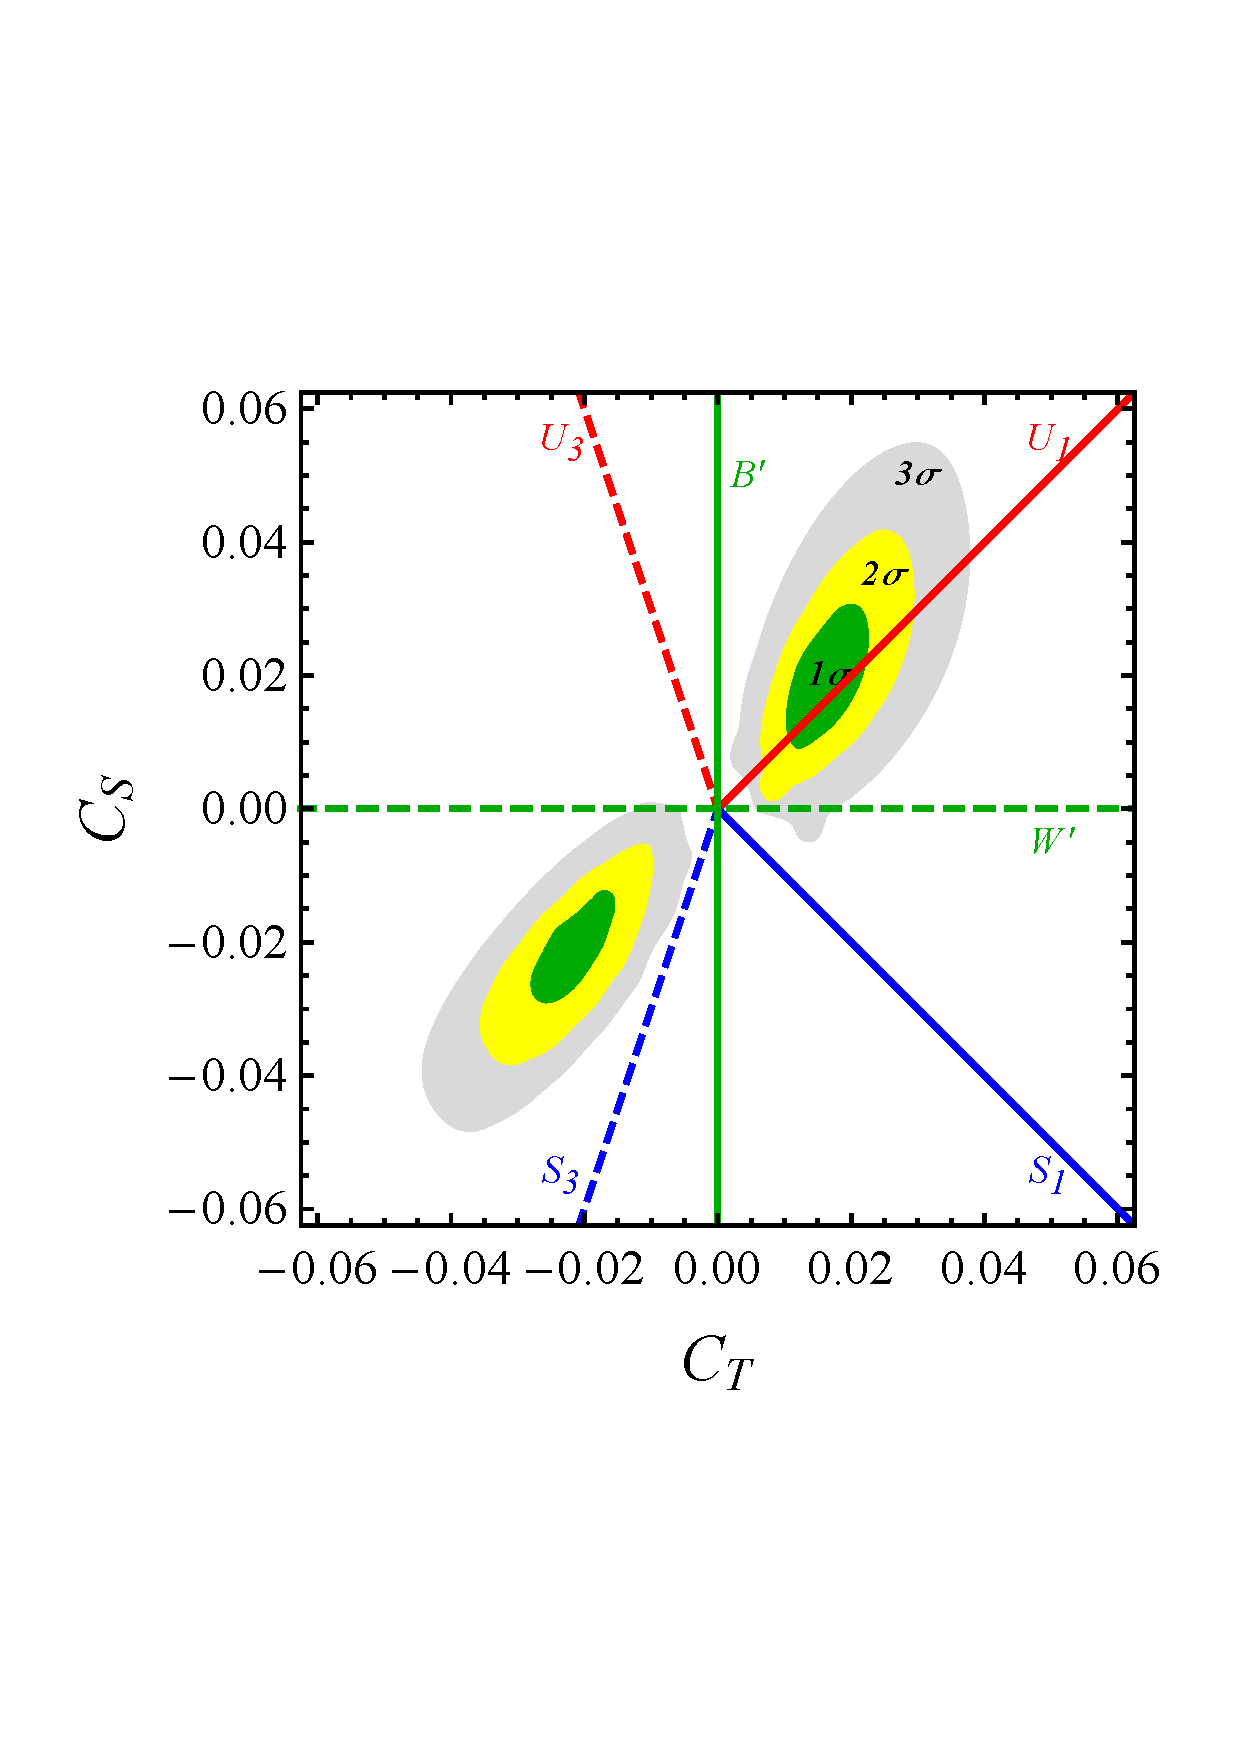
\includegraphics[width=0.75\textwidth]{SMS_fit.pdf} 
      \vspace*{-30mm}
   \caption{Fit of the coefficients $C_T$ and $C_S$ in Eq. \ref{eq:leff} from flavour physics observables. 
   	The parameters $\lambda^q_{sb}$ and  $\lambda^l_{\mu\mu}$ have been marginalised over. 
   	The green, yellow, and grey regions show the 1, 2, and 3$\sigma$ contours, respectively. 
   	Also shown as the straight lines are the correlations between $C_T$ and $C_S$, as predicted in various simplified models with a single mediator: colour-less vectors are shown in green, coloured scalars in blue, and coloured vectors in red. 
   	Electroweak singlet mediators are shown as solid lines, triplets as dashed lines. 
   	From \citep{Buttazzo:2017ixm}.}
\label{fig:fit}
\end{center}
\end{figure}

% =======
\subsection{Simplified Models}
\label{sec:B-SimMod}

The allowed regions in $C_T$ and $C_S$ from the EFT results are not
transparent in terms of an underlying physics idea. However,
they can both be
interpreted as new interactions in a \emph{Stage 3} SM-EFT and can be related
to elements of the concrete BSM models of Sect.~\ref{sec:B-con-BSM} in
a simplified model approach.  As discussed in Sect.~\ref{sec:SimpMod},
the idea of simplified models is to focus on just part of a BSM model, say a
single type of particle and evaluate its constraints and potential
consequences. This approach starts from a Lagrangian consisting of the
SM and a term representing a hypothetical new particle with a free
coupling strength.  The outcome of this Lagrangian is then matched to
Eq.~\ref{eq:leff}.
% The four-fermion operators in Eq. (\ref{eq:leff}) are induced by the exchange of a new heavy particle. 
Assuming $B'(1,1,0)$ or $W'(1,3,0)$; (colour-triplet scalar particles)
$S_1(\bar{3},1,1/3)$ or $S_3(\bar{3},3,1/3)$; (colour-triplet vector
particles), $U_1^\mu(3,1,2/3)$ or $U_3^\mu(3,3,2/3)$\footnote{The
  numbers in brackets indicate the colour, weak, and hypercharge
  quantum numbers.}, one obtains a certain correlation between $C_T$
and $C_S$, shown as straight lines in Fig.~\ref{fig:fit}.  While in
these simplified forms the particles are only defined by their quantum
numbers, they could be interpreted as new electroweak bosons, scalar
or vector leptoquarks, which already were discussed in the context of
concrete BSM models.  Comparing the analysis performed within the
EFT, and the predictions of the different
simplified models, the model with a coloured vector mediator,
$U_1^\mu(3,1,2/3)$, is clearly preferred. 

